\begin{example}
    Consider the following network where we want to check a blacklist
    property, i.e. no packets arrive at $d$:
    \begin{center}
        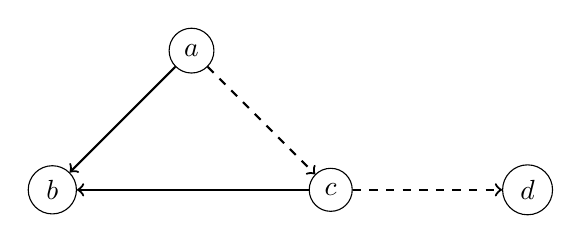
\begin{tikzpicture}[node distance={25mm},
                main/.style = {draw, circle},
                s/.style = {->,thick},
                d/.style = {->,thick,dashed} ]
            \node[main] (b) {$b$};
            \node[main] (a) [above right of=b] {$a$};
            \node[main] (c) [below right of=a] {$c$};
            \node[main] (d) [right of=c] {$d$};
            \draw[s] (a) -- (b);
            \draw[d] (a) -- (c);
            \draw[s] (c) -- (b);
            \draw[d] (c) -- (d);
        \end{tikzpicture}
    \end{center}
    We define this network using the following DyNetKAT term:
    \begin{align*}
        S_{xy}  & = l = x \cdot l \la y              \\
        P       & = u!S_{ac}                         \\
        Q       & = u!S_{cd}                         \\
        N_{x,y} & = (S_x+S_y)^* \oplus u?x';N_{x',y}
        \oplus u?y';N_{x,y'}                         \\
        SDN     & = N_{ab,cb} \parallel P \parallel Q
    \end{align*}
    We may rewrite the terms as follows:
    \begin{align*}
        N_{ab,cb} & = (S_{ab} + S_{cb})^* \oplus u?S_{ac};N_{ac,cb}
        \oplus u?S_{cd};N_{ab,cd}                                   \\
        N_{ac,cb} & = (S_{ac}+S_{cb})^* \oplus u?S_{cd};N_{ac,cd}   \\
        N_{ab,cd} & = (S_{ab}+S_{cd})^* \oplus u?S_{ac};N_{ac,cd}   \\
        N_{ac,cd} & = (S_{ac}+S_{cd})^*
    \end{align*}
    Given a packet $\sigma$ where $\sigma(l) = a$ we can replace NetKAT
    policies with actions of the form $(\sigma, \sigma')$.
    In this network we denote the action $(\sigma, \sigma')$
    with $xy$ where $\sigma(l) = x$ and $\sigma'(l) = y$.
    Let $N'_{x,y}$ be the term where we replaced NetKAT policies with
    actions of the form $(\sigma,\sigma')$ and let we use $p,p',q,q'$ to
    denote the actions $u?S_{ac},u!S_{ac},u?S_{cd},u!S_{cd}$.
    Thus we have:
    \begin{align*}
        SDN & = N'_{ab,cb} \parallel P \parallel Q \\
        P & = p' \\
        Q & = q' \\
        N'_{ab,cb} & = ab \oplus p;N'_{ac,cb} \oplus q;N'_{ab,cd} \\
        N'_{ac,cb} & = ac \oplus ab \oplus q;N'_{ac,cd}   \\
        N'_{ab,cd} & = ab \oplus p;N'_{ac,cd}             \\
        N'_{ac,cd} & = ac \oplus ad 
    \end{align*}
    Now, we wish to derive the event structure of the $SDN$.
    We consider $\oplus, ;, \parallel$ operators in DyNetKAT as 
    $+,\cdot,\times$ operators in the language respectively.

    \begin{align*}
        \sem{P} & = (\s{p'},\e,\s{\e \vdash p'}) \\
        \sem{Q} & = (\s{q'},\e,\s{\e \vdash q'}) \\
        \sem{P \parallel Q} & = (\s{p',q'},\e, \s{\e \vdash p',\e \vdash q'}) \\
        \sem{N'_{ac,cd}} &= 
        (\s{ac,ad},\s{ac \# ad}, \s{\e \vdash ac, \e \vdash ad}) \\
        \sem{p;N'_{ac,cd}} & = 
        (\s{p,ac,ad},\s{ac \# ad},\s{\e \vdash p, p \vdash ac, p \vdash ad}) \\
        \sem{ab\oplus p;N'_{ac,cd}} & =
        (\s{p,ab,ac,ad}, \s{ab\#p,ab\#ac,ab\#ad,ac\#ad}, \\
        & \s{\e \vdash ab, \e \vdash p, p \vdash ac, p \vdash cd}) \\
        \sem{q;N'_{ac,cd}} & = (\s{q,ac,ad},\s{ac\# ad},
        \s{\e \vdash q, q \vdash ac, q \vdash ad} \\
        \sem{ab \oplus q;N'_{ac,cd}}  & = (\s{q,ab,ac,ad},
         \s{ac \# ad, ab\# q,ab\#ac, ab \# ad, },\\
         & \s{\e \vdash ab, \e \vdash q, q \vdash ac, q \vdash ad} ) \\
        \sem{ac \oplus ab \oplus q;N'_{ac,cd}}  & = (\s{q,ab,ac_1,ac_2,ad}, \\
        & \s{ac_1 \# ad, ab\# q,ab\#ac_1, ab \# ad,
            ac_2 \# ab, ac_2 \# q, ac_2 \# ac_1, ac_2 \# ad
         },\\
         & \s{\e \vdash ab, \e \vdash q, q \vdash ac_1, q \vdash ad, 
         \e \vdash ac_2} ) \\
        \sem{q;N'_{ab,cd}} & =
        (\s{p,q,ab,ac,ad}, \s{ab\#p,ab\#ac,ab\#ad,ac\#ad}, \\
        & \s{\e \vdash q, q \vdash ab, q \vdash p, \s{p,q} \vdash ac,
        \s{p,q} \vdash cd}) \\
        \sem{p;N'_{ac,cb}}  & = (\s{p,q,ab,ac_1,ac_2,ad}, \\
        & \s{ac_1 \# ad, ab\# q,ab\#ac_1, ab \# ad,
            ac_2 \# ab, ac_2 \# 1, ac_2 \# ac_1, ac_2 \# ad
         },\\
         & \s{\e \vdash p, \s{p} \vdash ab, \s{p} \vdash q, 
         \s{p,q} \vdash ac_1, \s{p,q} \vdash ad, \s{p} \vdash ac_2} ) \\
         \sem{ p;N'_{ac,cb} \oplus q;N'_{ab,cd}} & = (
        \s{p_1,p_2,q_1,q_2,ab_1,ab_2,ac_{21},ac_{22},ac_1,ad_1,ad_2}, \\
         & \s{ab_1\#p_1,ab_1\#ac_1,ab_1\#ad_1,ac_1\#ad_1 \\
         & ac_{21} \# ad_2, ab_2\# q_2,ab_2\#ac_{21}, ab_2 \# ad_2, \\
         & ac_{22} \# ab_2, ac_{22} \# q_2, ac_{22} \# ac_{21}, 
         ac_{22} \# ad_2 } \\
         & \cup \s{e_{i}\#e_{i'}| i \neq i' } \\
         & \s{\e \vdash p_2, \s{p_2} \vdash ab_2, \s{p_2} \vdash q_2, 
         \s{p_2,q_2} \vdash ac_{21}, \s{p_2,q_1} \vdash ad_2, \s{p_2} 
         \vdash ac_{22},  \\
        & \e \vdash q_1, q_1 \vdash ab_1, q_1 \vdash p_1, 
        \s{p_1,q_1} \vdash ac_1, \s{p_1,q_1} \vdash cd_1}) \\
        \sem{ab \oplus p;N'_{ac,cb} \oplus q;N'_{ab,cd}} & = (
        \s{p_1,p_2,q_1,q_2,ab_1,ab_2,ab_3,ac_{21},ac_{22},ac_1,ad_1,ad_2}, \\
         & \s{ab_1\#p_1,ab_1\#ac_1,ab_1\#ad_1,ac_1\#ad_1 \\
         & ac_{21} \# ad_2, ab_2\# q_2,ab_2\#ac_{21}, ab_2 \# ad_2, \\
         & ac_{22} \# ab_2, ac_{22} \# q_2, ac_{22} \# ac_{21}, 
         ac_{22} \# ad_2 } \\
         & \cup \s{e_{i}\#e_{i'}| i \neq i' } \\
         & \s{\e \vdash p_2, \s{p_2} \vdash ab_2, \s{p_2} \vdash q_2, 
         \s{p_2,q_2} \vdash ac_{21}, \s{p_2,q_1} \vdash ad_2, \s{p_2} 
         \vdash ac_{22},  \\
        & \e \vdash ab_3, \e \vdash q_1, q_1 \vdash ab_1, q_1 \vdash p_1, 
        \s{p_1,q_1} \vdash ac_1, \s{p_1,q_1} \vdash cd_1}) \\
    \end{align*}
\end{example}